% !TEX root = Kreisfahrt.tex
\section{Mathematik zur Kinematik / Dynamik}
\begin{figure}
    \centering
    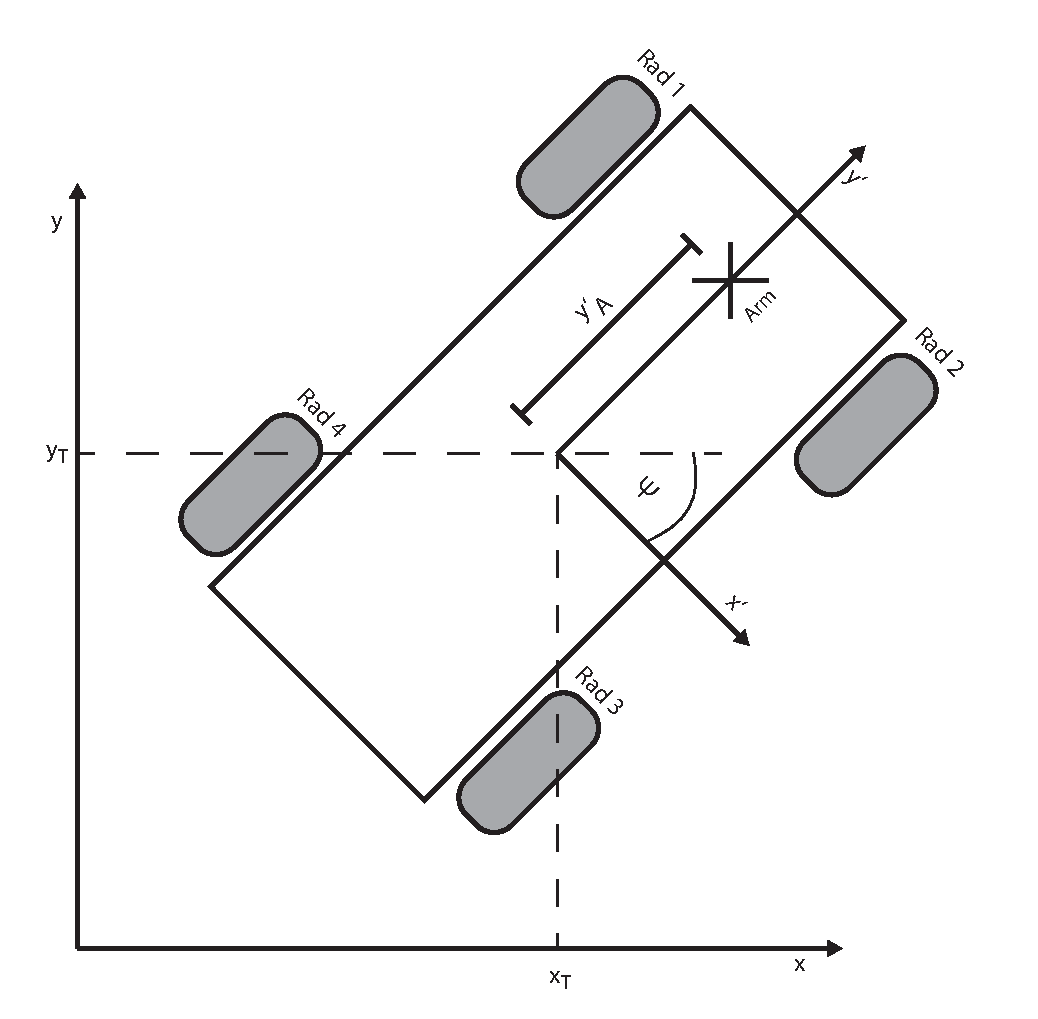
\includegraphics[width=.8\textwidth]{Abbildungen/Koordinaten}
    \caption{Bezugskoordinaten}
\end{figure}
Dieses Kapitel beschreibt die Mathematik hinter der Kinematik und Dynamik des Mecanum-Roboters.
Jede Bewegung setzt sich aus einer translatorischen und einer rotatorischen Bewegung zusammen.

\subsection{Translation}
Vereinfacht kann die translatorische Bewegung des Mecanum-Roboters durch die Drehrichtung und Drehgeschwindigkeit der Mecanum-Räder beschrieben werden. Abhängig von den unterschiedlichen Kombination fährt der Roboter entlang des Vektors für die Gesamtbewegung.
\begin{figure}[H]
    \centering
    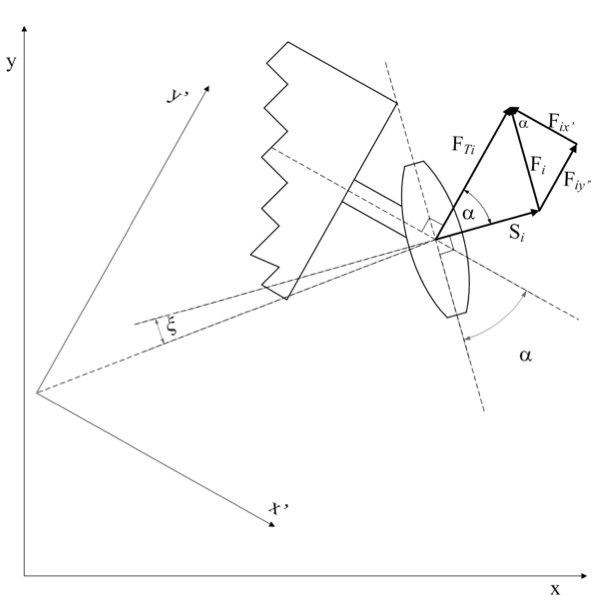
\includegraphics[width=.6\textwidth]{Abbildungen/Kraefte-am-Rad}
    \caption{Kräftegleichgewicht an einem Mecanum-Rad.}
\end{figure}

Die Leistung einer vektoriellen Kraft berechnet sich nach:
$$ P_F = F_T \cdot v_F $$

Wirken Kraft und Geschwindigkeit entlang einer Koordinatenachse, haben beide Vektoren die gleiche Komponente ungleich null und ihr Skalarprodukt kann vereinfacht als Produkt der skalaren Größen betrachtet werden.

Die Kraftvektor in $x$- und $y$-Richtung setzt sich zusammen als die Summe der einzelnen $x$- und $y$-Vektoren der vier Räder:
\begin{align*}
    \sum_{i=1}^4 F_{iy} &= \sum_{i=1}^4 F_i \sin \alpha                 \\
    &= \sum_{i=1}^4 SIG \cdot K_i F_{Ti} \sin^2 \alpha                  \\
    &= \sum_{i=1}^4 SIG \cdot \frac{1}{2} K_i F_{Ti}                    \\
    \sum_{i=1}^4 F_{ix} &= \sum_{i=1}^4 F_i \cos \alpha                 \\
    &= \sum_{i=1}^4 (-1)^i SIG \cdot K_i F_{Ti} \sin \alpha \cos \alpha \\
    &= \sum_{i=1}^4 (-1)^i SIG \cdot \frac{1}{2} K_i F_{Ti}             \\
\end{align*}

SIG steht als Vorzeichenkonventionen für die Drehrichtung der Räder. Diese werden in der Steuerung direkt implementiert und werden daher bei den folgenden Rechnungen nicht weiter betrachtet.

Der Winkel $ \alpha $ liegt zwischen den Drehachsen der Rollen und der Räder ($\alpha = 45^\circ$).
Für eine translatorisch Bewegung müssen sich jeweils die diagonalen Räder (1, 3 und 2, 4) mit derselben Geschwindigkeit drehen. Entsprechen müssen ihre Kraftvektoren $F_{T1, 3} / F_{T2, 4}$ gleich groß sein.
Durch Auflösen der Summenzeichen erhält man ein Gleichungssystem:
\begin{align*}
    F_x &= - K_i F_{T1, 3} + K_i F_{T2, 4} \\
    F_y &= K_i F_{T1, 3}   + K_i F_{T2, 4}
\end{align*}

Nach Umstellen erhält man $F_{T1, 3}$ und $F_{T2, 4}$ und kann somit auch direkt die Geschwindigkeiten berechnen:
\begin{align*}
    F_{T1, 3} &= \frac{F_y + F_x}{K_i} &\Rightarrow v_{T1, 3} &= \frac{v_y + v_x}{K_i} \\
    F_{T2, 4} &= \frac{F_y - F_x}{K_i} &\Rightarrow v_{T2, 4} &= \frac{v_y - v_x}{K_i} \\
\end{align*}

Der Faktor $K_i$ setzt sich aus unterschiedlichen Faktoren zusammen, welche die durch das Motormoment erzeugten treibenden Kräfte beeinflussen und wird für den Boden der Werkstatt empirisch ermittelt.


\subsection{Rotation}
Die Rotation des Mecanum-Roboters um sein Zentrum kann durch die Drehrichtung der Räder bei gleicher Geschwindigkeit beschrieben werden.
Für eine Drehung im Uhrzeigersinn drehen Rad 1 und 2 rückwärts, Rad 3 und 4 vorwärts. Für eine Drehung gegen den Uhrzeigersinn entsprechend umgekehrt.
\begin{align*}
    v_{ref} &= K_i \cdot r \cdot \omega \\
    v_1 = v_4 &= - v_{ref}              \\
    v_2 = v_3 &= + v_{ref}
\end{align*}


\subsection{Koordinatentransformation}
Dieses Kapitel befasst sich mit der Koordinatentransformation vom ortsfesten Bezugskoordinatensystem zum Koordinatensystem des Mecanum-Roboters. \\
Die translatorische Verschiebung wird durch den Vektor $\underline T$ beschrieben.
\begin{align*}
\underline T =
\begin{bmatrix}
x_{T}\\
y_{T}\\
0
\end{bmatrix}
\end{align*}
Rotationsmatrix $\underline R$ um den Gierwinkel $\Psi$.
\begin{align*}
 \underline R_{\Psi} =
\begin{bmatrix}
  \cos{\Psi} & -\sin{\Psi} & 0\\
  \sin{\Psi} & \cos{\Psi} & 0\\
  0 & 0 & 1
\end{bmatrix}
\end{align*}
Positionsvektor des Roboter $\underline P$.
\begin{align*}
\underline P = \underline R_{\Psi} \cdot \underline T =
\begin{bmatrix}
  \cos{\Psi} & -\sin{\Psi} & 0\\
  \sin{\Psi} & \cos{\Psi} & 0\\
  0 & 0 & 1
\end{bmatrix}\cdot
\begin{bmatrix}
x_{T}\\
y_{T}\\
0
\end{bmatrix}=
\begin{bmatrix}
x_{T} \cdot \cos{\Psi}-y_{T} \cdot \sin{\Psi}\\
x_{T} \cdot \sin{\Psi}+y_{T}  \cdot \cos{\Psi}\\
0
\end{bmatrix}
\end{align*}
Als Ergänzung wird die Transformation bis zum Koordinatenursprung des montierten Roboterarms weitergeführt.
\begin{align*}
\underline T_{A} + \underline P =
\begin{bmatrix}
x_{A} + x_{T} \cdot \cos{\Psi}-y_{T} \cdot \sin{\Psi}\\
y_{A} + x_{T} \cdot \sin{\Psi}+y_{T}  \cdot \cos{\Psi}\\
z_{A}
\end{bmatrix}
\end{align*}